\documentclass[12pt]{article}
\usepackage[utf8]{inputenc}
\usepackage{style}

\title{Oracle Quantum Computing}
\author{Joshua Spayd}
\date{\today}

\begin{document}
\maketitle

\section{Introduction}
It is the objective of the theoretical sciences to develop mathematical models
that describe natural phenomena, and when faced with a result that contradicts
existing models, it is the responsibility of the theorist to augment these
models to reconcile with the observed phenomena, and to resolve
inconsistencies across scientific theories. The strong Church-Turing thesis
conjectures that every physically realizable computation model can be
simulated by a Turing machine with polynomial overhead in runtime, but
physicist Richard Feynman \cite{Fey82} notes that the obvious classical
algorithm for simulating a quantum system of $n$ particles runs exponentially
in $n$ and suggests that computers be equipped with quantum mechanical gates
in order to enable efficient simulation of quantum systems. If quantum systems
cannot be efficiently simulated by Turing machines --- and if general-purpose
quantum computers are physically realizable --- then the strong Church-Turing
thesis is false, and we require a new model of computation. Though questions
of the feasibility and relative efficiency of quantum computers are yet
unanswered, this uncertainty has not prevented theorists from developing
quantum computational models. In this paper, we will formalize quantum computing
and quantum oracles, and then we will describe a few results from quantum
complexity theory, with emphasis on the result from \cite{BB92} that relative to
certain oracles, quantum computers are more powerful than nondeterministic
computers, or in the words of  Berthiaume and Brassard, that ``quantum can beat
nondeterminism.''


\section{Quantum mechanics}
\begin{figure}[H]
  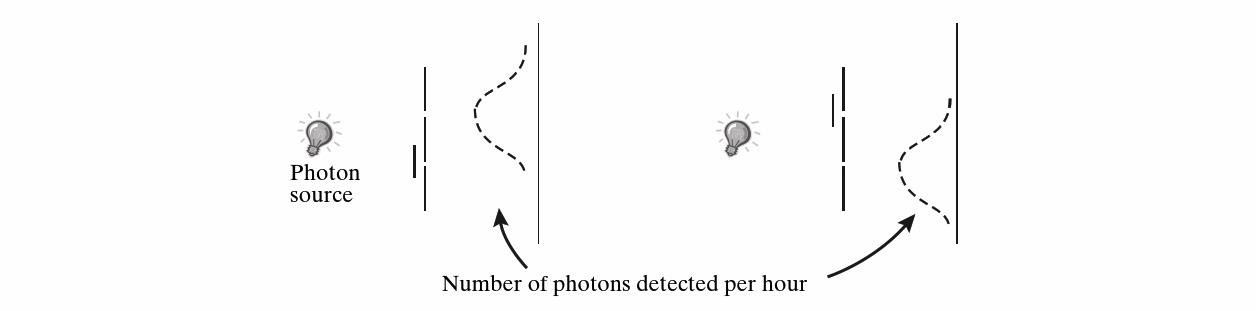
\includegraphics[width=\textwidth]{two-slit-1}
  \caption{\cite[p. 203]{AB09}}
  \label{fig:two-slit-1}
\end{figure}
\begin{figure}[H]
  
\includegraphics[width=\textwidth]{two-slit-2}
  \caption{\cite[p. 203]{AB09}}
  \label{fig:two-slit-2}
\end{figure}


\section{Modeling quantum computation}

\subsection{Quantum operations}
\begin{defn}[Quantum operation {\cite[p. 210]{AB09}}]
  \label{defn:op}
  A \emph{quantum operation} for an $m$-qubit register is a funciton $F :
  \CC^{2^m} \to \CC^{2^m}$ that maps its previous state to the new state and
  satisfies the following conditions:
  \begin{adjustwidth}{0.25in}{0in}
    \emph{Linearity:} $F$ is a linear function. That is, for every $\vec{v} \in
    \CC^{2^n}$, $F(\vec{v}) = \sum_x \vec{v}_x F(\reg*{x})$. \\
    \emph{Norm preservation:} $F$ maps unit vectors to unit vectors. That is,
    for every $\vec{v}$ with $\norm*{\vec{v}}_2=1$, $\norm*{F(\vec{v})}_2=1$.
  \end{adjustwidth}
\end{defn}

\subsection{Quantum Turing machines and the class $\BQP$}
\begin{defn}[Quantum computation and the class $\BQP$ {\cite[p. 213]{AB09}}]
  \label{defn:bqp}
  Let $f : \zo^* \to \zo$ and $T : \NN \to \NN$ be some functions. We say that
  $f$ is \emph{computable in quantum $T(n)$-time} if there is a polynomial-time
  classical TM that on input $\paren*{1^n, 1^{T(n)}}$ for any $n \in \NN$
  outputs the descriptions of quantum gates $F_1, \dots, F_T$ such that for
  every $x\in \zo^n$, we can compute $f(x)$ with probability at least
  $\nfrac{2}{3}$ by the following process:
  \begin{enumerate}
    \item Initialize an $m$-qubit quantum register to the state
      $\reg*{x0^{n-m}}$ (i.e., $x$ padded with zeroes), where $m \le T(n)$.
    \item Apply ons after the other $T(n)$ elementary quantum operations $F_1,
      \dots, F_T$ to the register.
    \item Measure the register and let $Y$ denote the obtained value. (That is,
      if $\vec{v}$ is the final state of the register, then $Y$ is a random
      variable that takes the value $y$ with probability $\abs*{\vec{v}_y}^2$
      for every $y \in \zo^m$.)
    \item Output $Y_1$.
  \end{enumerate}
  A Boolean function $F : \zo^* \to \zo$ is in $\BQP$ if there is some
  polynomial $p : \NN \to \NN$ such that $f$ is computable in quantum
  $p(n)$-time.
\end{defn}

\begin{thm}
  $\BPP \subseteq \BQP$.
\end{thm}

\begin{thm}
  $\BQP \subseteq \PSPACE$.
\end{thm}

\begin{conj}
  $\NP \not\subseteq \BQP$.
\end{conj}

\begin{thm}[\cite{BBBV97}]
  Relative to an oracle chosen uniformy at random, with probability 1, the class
  $\NP$ cannot be solved on a quantum Turing machine in time $\smallo{2^{n/2}}$.
\end{thm}
``There is no black-box approach to solving $\NP$-complete problems using some
uniquely quantum features of QTMs.''

\begin{conj}
  $\BPP \subsetneq \BQP$.
\end{conj}

\begin{thm}[\cite{Sho97}]
  $\lang{Factoring} \in \BQP$.
\end{thm}

\begin{thm}[\cite{BB92}]
  Under appropriate oracles, there is a decision problem that can be solved in
  polynomial time on a quantum computer that would require exponential time on a
  classical nondeterministic computer.
\end{thm}
``Quantum can beat nondeterminism.''

\section{Quantum oracles}
\TODO{Refer to {\cite{BBBV97}}.}


\section{Quantum can beat nondeterminism \cite{BB92}}


\nocite{*}
\bibliographystyle{alpha}
\bibliography{bibliography}
\end{document}
